\documentclass[aps]{revtex4}
\usepackage{natbib}
\usepackage{graphics} % use the graphics package for simple commands
\usepackage{graphicx}
\usepackage{amsmath}
\usepackage{amssymb} % The amssymb package provides various useful mathematical symbols
\usepackage{fdsymbol}
\usepackage{wrapfig}

\usepackage{pstricks}
%\usepackage{cite}

\usepackage[symbol]{footmisc}
\renewcommand{\thefootnote}{\fnsymbol{footnote}}

\newcommand{\ket}[1]{\ensuremath{\left| #1 \right\rangle}}
\newcommand{\bra}[1]{\ensuremath{\left\langle #1 \right|}}
\newcommand{\braket}[2]{\ensuremath{\left\langle #1 \right|\left. #2 \right\rangle}}
\newcommand{\expect}[1]{\ensuremath{\left\langle #1 \right\rangle}}
\newcommand{\eV}{\mbox{eV}}
\newcommand{\icm}{\ensuremath{\mbox{cm}^{-1}}}
\newcommand{\cm}{\mbox{cm}}
\newcommand{\EE}[1]{\ensuremath{\times 10^{ #1 }}}
\newcommand{\ee}[1]{\ensuremath{\times 10^{ #1 }}}
\newcommand{\norm}[1]{\ensuremath{\left| #1 \right|}}
\newcommand{\abs}[1]{\ensuremath{\left| #1 \right|}}
\newcommand{\HH}{\mathcal{H}}
\newcommand{\laplace}[1]{\ensuremath{\mathcal{L}\left\{ #1 \right\}}}
\newcommand{\fourier}[1]{\ensuremath{\mathcal{F}\left\{ #1 \right\}}}
\newcommand{\invlaplace}[1]{\ensuremath{\mathcal{L}^{-1}\left\{ #1 \right\}}}
\newcommand{\invfourier}[1]{\ensuremath{\mathcal{F}^{-1}\left\{ #1 \right\}}}
\newcommand{\myexp}[1]{\ensuremath{ \exp\left( #1 \right) }}
\newcommand{\eps}{\varepsilon}
\newcommand{\myerf}[1]{\ensuremath{{\mathrm{erf}\left( #1 \right)}}}
\newcommand{\heaviside}[1]{\ensuremath{ \mathrm{\Theta}\left( #1 \right)}}
\newcommand{\etal}{,~\textit{et~al.,~}}


\usepackage{times}

\graphicspath{{./figs/}} % Change Graphics Path for figs and institution logo.

\begin{document}
%---- Set up title section ----%

\title{The CookieBox and Edge Machine Learning}

\author{Audrey Corbeil-Therrien\footnotemark, Debadri Das\footnotemark, Matt Feldman\footnotemark, \setcounter{footnote}{0} Averell Gatton\footnotemark, Kunle Olukotun\setcounter{footnote}{2}\footnotemark, Amedeo Perazzo\setcounter{footnote}{0}\footnotemark, Omar Quijano\setcounter{footnote}{0}\footnotemark, Peter Walter\setcounter{footnote}{0}\footnotemark, and Ryan N. Coffee\setcounter{footnote}{0}\footnotemark \setcounter{footnote}{3}\footnotemark\\
\setcounter{footnote}{0}\footnotemark LCLS \hspace{24pt} \footnotemark Stanford Applied Physics \hspace{24pt} \footnotemark Stanford EE/CS \hspace{24pt}\footnotemark The PULSE Institute, SLAC National Accelerator Lab, 2575 Sand Hill Road, Mail Stop 20, Menlo Park, California 94025}

\setlength{\parindent}{.05\linewidth}



%---- Can't use the figure environment within multicolumns. Set up our own counter for figures. ----%
%---- Also, set up the \figwidth length ----%

\newcounter{figscount}
\newlength{\figwidth}
\setlength{\figwidth}{.9\linewidth}


%---- Abstract ----%
\begin{abstract}
We present an update of two interrelated projects, the angle resolving electron time-of-flight spectrometer array known as ``The CookieBox'' and the detector readout and analysis chain that is the target for on-going research into high efficiency machine learning for detector-local streaming data analysis known as ``EdgeML.''
These two efforts are being pursued in parallel via a co-design approach to this quintessential LCLS-II diagnostic and spectroscopic detector system.
\end{abstract}


%\maketitle

%---- Body ----%
\section{Introduction}
\section{Mechanical Design}
\section{Electrical Design}
\section{Data Pipeline}

Motivating co-design, we look for a pipelined algorithm that fits into the spare digitizer FPGA logic that also relaxes our need to record multiple electron hits in so-called ``current'' mode.

\begin{wrapfigure}[40]{r}{.5\linewidth}
\centerline{\includegraphics[clip,width=\linewidth]{dynamic.kernel.motivation.eps}}
\caption{\label{fig::kde}
Here we show Kernel Desity Estimation (KDE) in blue by varying the bandwidth the kernel that is applied to the electron hits associated with the under-sampled probability distribution functions (PDFs), shown as red, as described in the text.
}
\end{wrapfigure}

\begin{figure}
\centerline{\includegraphics[clip,width=\figwidth]{dynamic.kernel.motivation.multi.eps}}
\caption{\label{fig::multi_single_kde}
Here we compare the case of multiple (5) shots averaged together (left) with single shot cases with undersampled probability distrbutions (center and right).
}
\end{figure}

\section{Conclusion}
\section*{The CookieBox}

The CookieBox project is a recently funded (FY19-FY20) project under the DOE Accelerator and Detectors Research program.
This project, formally titled ``Enabling long wavelength streaking for attosecond x-ray science'' aims to produce a prototype detector system that demonstrates an optimal balance between electron time-of-flight (ToF) spectral resolution and collection efficiency.
The detector is optimized for attosecond angular streaking \cite{Nick2018,Siqi2018} for x-ray pulse characterization at full LCLS-II repetition rates.
The output of this project will feed the design specifications for the ``Multi-Resolution CookieBox Optimized for Future Free Electron Experiments'' (MRCOFFEE) end-station led by Peter Walter for the Hutch 1.1.
The final goal is therefore attosecond resolving x-ray pulse characterization that can be used for on-line sort and veto data routing decisions for downstream detectors.

\noindent\centerline{
%\begin{minipage}[t]{\figwidth}
\begin{minipage}[t]{.6\linewidth}
\includegraphics[clip,width=.9\linewidth]{Composite_Ave.ps}
\end{minipage}
\begin{minipage}[b]{.4\linewidth}
\addtocounter{figscount}{1}
\manuallabel{fig::Potentials}{\arabic{figscount}}
{\small Figure \arabic{figscount}. (top) Potential field for one eToF module planned for the CookieBox detector array.
(bottom) Detail of module showing equipotential field lines in red.}
\end{minipage}
}

Figure~\ref{fig::Potentials} shows a preliminary design for the ToF modules, the first of which are currently being developed with engineering staff.
To preserve the high-time resolution of the Hamamatsu F9890-32 Micro-Channel Plates (MCPs) we have chosen the Abaco FMC134 FPGA Mezzanine Card waveform digitizer. 
This card will provide 2 channels each of 12 bit depth data rate with 6.4 GS/s.
The Hamamatsu waveform is shown in Fig.~\ref{fig::powerspec} (left as Fourier transform, right as waveform) and the corresponding FMC134 sampling is shown as red points in the inset.

\noindent\centerline{
\begin{minipage}[t]{\figwidth}
\centerline{\includegraphics[trim={-2cm -2cm 0 0 },width=.8\linewidth]{plotting.resampled.eps}}
\addtocounter{figscount}{1}
\manuallabel{fig::powerspec}{\arabic{figscount}}
{\small Figure \arabic{figscount}. (top) Power spectrum of the measured impulse response for the proposed Hamamatsu MCP stack.
(bottom) Impulse response function raw and Weiner filtered and compared in inset to the sampling for proposed LCLS-II Hutch 1.1 6 GSps digitizers.}
\end{minipage}
}

We use simulated time-energy distributions, represented here simply as individual points whose size and color represent the relative intensity of the sub-pulse and the x-y axes correspond to carrier-cycle and streak amplitude scaled time-energy distribution.
For simplicity we currently assume sub-pulses of well defined energy and time as shown center in Fig.~\ref{fig::ToFs}.
We draw a random sampling of approximately 50 electrons per angle distributed according to the simulated ToF probability distribution function (PDF).
Individual electrons are represented at left in Fig.~\ref{fig::ToFs} as points radiating from the center with radius equal to time-of-Flight in nanoseconds and corresponding angle according to the 16 channels of the CookieBox.
These individual electrons are then convolved with an ensemble of measured MCP response functions to produce the ``forward simulation'' signals at right in Fig.~\ref{fig::ToFs}.
%At right we see the resulting signal waveforms after convolution with the measured Hamamatsu response and noise, thus the last stage of our ``forward simulation.''
These ``forward simulation'' signals provides the ``input data'' that corresponds to the ``ground truth'' the time-energy distribution.
We can now pursue machine learning algorithms to solve the inverse problem to converge on a model for interpreting measured signals.

\begin{figure}
\centerline{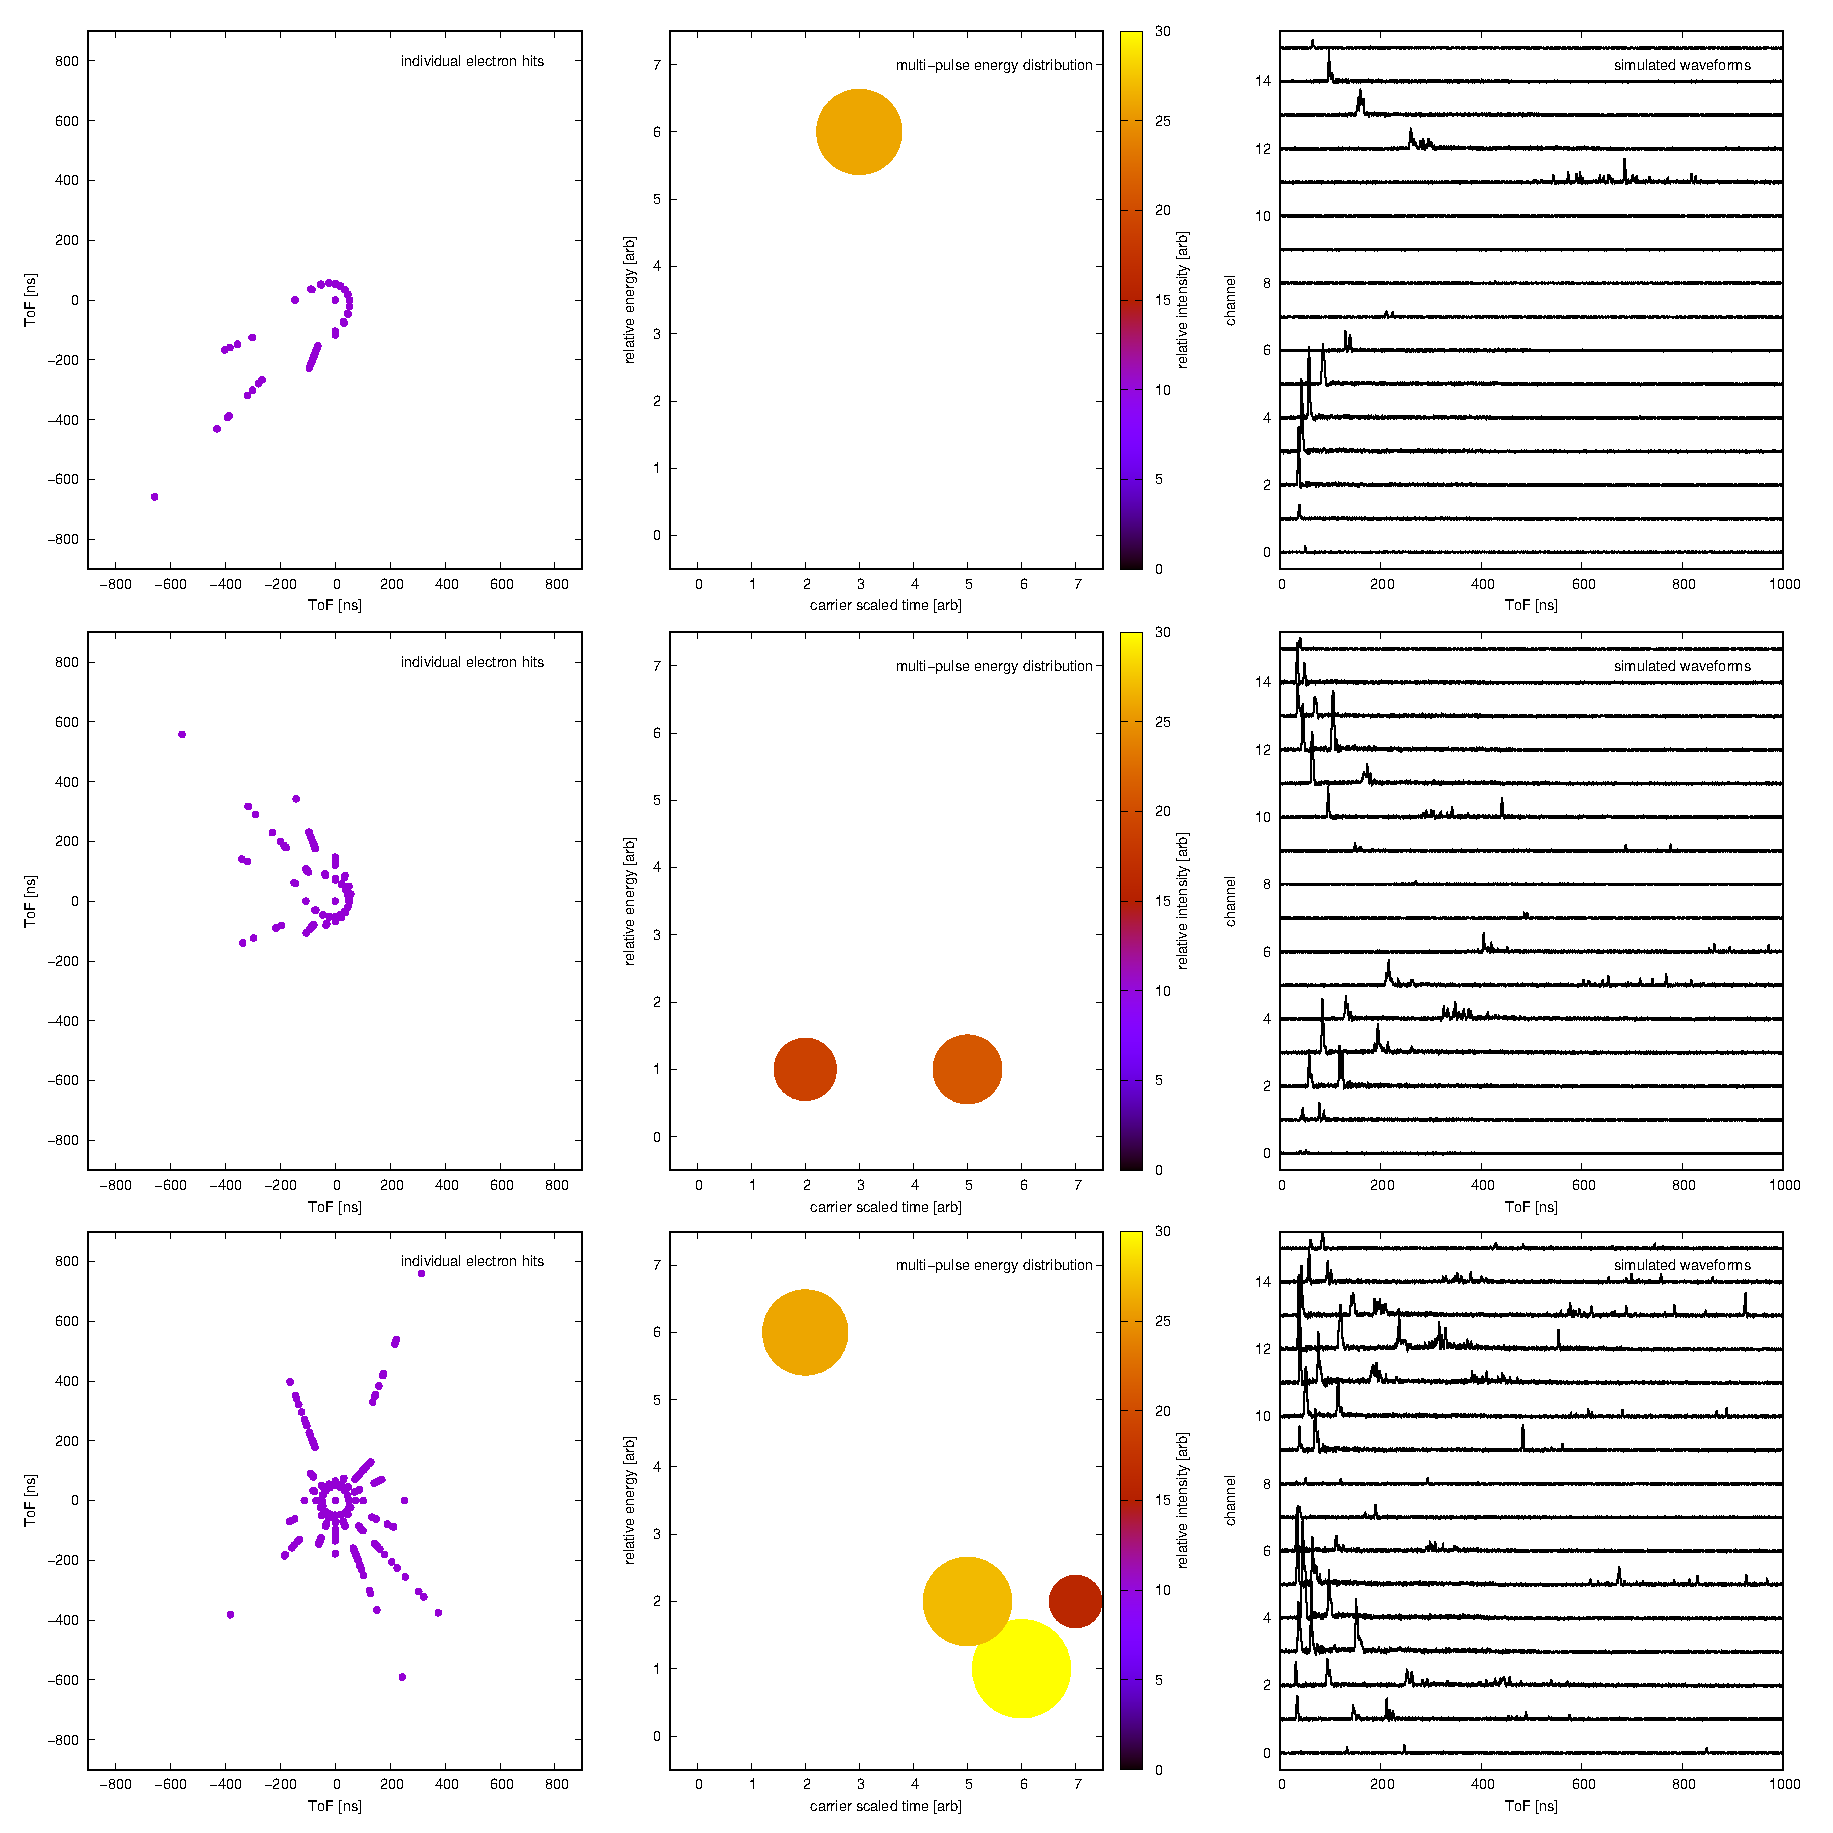
\includegraphics[trim={-2cm -2cm 0 0},width=\figwidth]{plotting.ToFs.eps}}
\caption{\label{fig::ToFs}
	(left) Electron arrival times in polar coordinates.
	(center) Multi-pulse time-energy (x-y) distributions of the x-ray pulses (point size and color indicate relative intensity).
	(right) Simulated ToF waveforms.
}
\end{figure}

In Ref.~\cite{Nick2018}, the previous generation of CookieBox was run in a 10s of electrons per shot counting regime in order that, given the much broader impulse response, the measured waveforms fairly closely represented the PDF for the outgoing photo-electrons.
A comparable hit-rate per shot was tested recently at the European XFEL, but for 1~MHz burst pulse rate which showed 10-fold signal degradation over the burst duration \cite{MarkusUpdate2019}.
Furthermore, we have chosen to increase the drift length in order to improve the spectral resolution over a broader energy window.
This increase in spectral resolution over a broader range of incoming electron energies has the draw back of poorer collection solid angle.
We also note that the high time-resolution Hamamatsu MCPs have a rather small 27~mm active area, thus even further restricting the collection angle.
We are therefore targeting a machine learning data analysis paradigm that is more amenable to under sampled PDFs.

\begin{figure}
\centerline{\includegraphics[trim={-3cm -2cm 1cm 1cm },clip,width=.8\figwidth]{plotting.debadri.eps}}
\caption{\label{fig::debadri}
Preliminary investigation into using Kernel Density Estimator.
% in order to quickly convert the under-sampled probability distribution function of photo-electrons to the desired input waveform for x-ray pulse shape inference.
}
\end{figure}

We are currently investigating Kernel Density Estimation (KDE) that could be implemented in the on-digitizer FPGA.
Ideally KDE would convert the sparsely sampled PDF for the outgoing photo-electrons into an estimated continuous form.
Represented in Fig.~\ref{fig::debadri}, one can easily see that in the ``pile-up'' regime where two distinct spectral features (red Gaussians) overlap, KDE results insufficiently represent the ``true'' PDF (red).
Our goal is to use machine learning to help jointly optimize the balance between x-ray pulse reconstruction accuracy and KDE bandwidth tuning in the pre-processing layer.

\section*{Edge Machine Learning}

Machine learning is a method of nonlinear curve fitting for very high dimensional data.
Well fitted models have been shown to be quite immune to (Gaussian) noise.
Although fitting the model, so-called ``training,'' is both data and simulation hungry and also computationally expensive and time-consuming, the application of the trained model involves a fairly straight forward sequence of matrix operations.
These matrix operations, the so-called ``inference,'' parallelize well under either GPU or FPGA instantiation. 
A portion of the raw data will be also transferred for use in model validation and subsequent re-training, and active models will be tightly bound to the data that they were used to produce.%, allowing for subsequent interrogation if there arises doubt regarding the quality of results.
Such near-detector FPGA-based inference engines we call Inference at the Edge or ``EdgeML.''

\vspace{24pt}
\noindent\centerline{
\begin{minipage}[t]{\figwidth}
\centerline{\includegraphics[clip,width=.8\figwidth]{ConnectionDiagram_cookiebox_humaninloop_new.eps}}
\addtocounter{figscount}{1}
\manuallabel{fig::humaninloop}{\arabic{figscount}}
{\small Figure \arabic{figscount}.  
Current architecture for FPGA-based machine learning models.  
Early layers pre-analyze individual ToF channels independently and in parallel.
Deeper layers merge the results into the actionable information such as multi-pulse energy, delay, and polarization.
}
\end{minipage}
}\vspace{24pt}

Given the expected data rates for the LCLS-II(-HE) facilities, there is a growing EdgeML effort inside of LCLS that also has begun to extend to SSRL, High Energy Physics, and observational astronomy.  
Industry at large is entering an age where the velocity of data streams are becoming prohibitively high for expected network channels.
Given the potential for the CookieBox digitizers to produce a continuous data rate of over 200 GB/s, we are using the CookieBox project as a prescient use case for EdgeML.
This Edge Machine Learning project began with LDRD funding in FY18 and continues through FY19.

\begin{eqnarray}
\left[S_0, S_1 \cdots S_n\right] &\stackrel{\textrm{FPGA}}{\Longmapsfrom}& N_{\textrm{el}} (t) \stackrel{\textrm{Detector}}{\Longmapsfrom} \textrm{Event} \nonumber\\
\Downarrow\hspace{1cm}&&\hspace{1cm} \vec{\alpha} \stackrel{\textrm{Human}}{\Longmapsfrom} \textrm{Exp. Conditions}\nonumber\\
\Downarrow\hspace{1cm}&&\hspace{1cm} \Downarrow\nonumber\\
\left[S_0, S_1 \cdots S_n\right] &\stackrel{\textrm{Software}}{\Longmapsto}& \left[\tau_0 ,\tau_1 \cdots \tau_m \right] , \vec{\alpha} \nonumber\\%\stackrel{\textrm{Human}}{\Longmapsfrom} \textrm{Exp. Conditions}\\
   & &\hspace{1cm}\Downarrow \textrm{Software}\nonumber\\
 \textrm{Physical model} \stackrel{\textrm{Human}}{\Longmapsfrom} \expect{\mathcal{O} \left(\vec{\alpha}\right)} &\stackrel{\textrm{Simulation}}{\Longmapsfrom}& \mbox{Hist}\left( \mathcal{O} , \vec{\alpha} \right) \label{eqn::oldschool}
\end{eqnarray}

In the traditional case of data processing (Eq.~\ref{eqn::oldschool}), there are multiple levels where users leverage abstracted software to process incoming signals.
Detectors feed into digitized waveforms ($\left[S_0, S_1 \cdots S_n\right]$) by FPGA, with possible simple modifications.
The FPGAs then hand over digital waveforms to CPU based algorithms that convert signals into extracted parameters ($\left[\tau_0 ,\tau_1 \cdots \tau_m \right]$).
These parameters get combined with experimental conditions ($\vec{\alpha}$) for subsequent increment of a histogram ($\mbox{Hist}\left( \mathcal{O} , \vec{\alpha} \right)$) that the user hopes will represent some expectation value for an observable ($\expect{\mathcal{O} \left(\vec{\alpha}\right)}$).
We, on the other hand, take inspiration from Fig.~\ref{fig::hackernoon}.

There has been great recent progress with both in porting simple algorithms to Application Specific Integrated Circuits (ASICs) as well as compiling trained inference models to Field Programmable Gated Arrays (FPGAs) \cite{spatial}.  
When looking to industry, we see a clear trend to low-power, heavily parallelized, streaming data analysis \cite{hackernoon}.
This is driven by the coming evolution to so-called Industry 4.0, or the Industrial Internet of things (IIoT).
We plan to leverage SLAC's long history in ASIC and FPGA design to incorporate the machine learning analysis paradigm into the detector-side electronics.

\noindent\centerline{
\begin{minipage}[t]{\figwidth}
\centerline{\includegraphics[clip,width=.8\linewidth]{hackernoon.ps}}
\addtocounter{figscount}{1}
\manuallabel{fig::hackernoon}{\arabic{figscount}}
{\small Figure \arabic{figscount}. 
Cartoon from \cite{hackernoon} representing the growing importance of Edge compute solutions like FPGAs and ASICs for processing intensive tasks (blockchain in this case).
}
\end{minipage}
}\vspace{24pt}

We expect that with sufficient model training one could move directly from raw signal to an updated representation of the physical observable $\expect{\mathcal{O} \left(\vec{\alpha}\right)}$ (Eq.~\ref{eqn::newschool})
Of course, such an analysis chain would require adaptability and thus will likely not fit completely into the on-detector FPGA.
We adopt a co-design approach, leveraging the particular strengths of each piece of computational hardware, e.g. ASICs an FPGAs on the sensor along with FPGAs and GPUs further along the data stream.

 \begin{eqnarray}
 &\textrm{Exp. Conditions}&\nonumber \\
   & \hspace{1cm}\Downarrow & \label{eqn::newschool}\\%\textrm{Detectors}\\
 \textrm{Physical model} \stackrel{\textrm{Human}}{\Longmapsfrom} \expect{\mathcal{O} \left(\vec{\alpha}\right)} \stackrel{\textrm{FPGA}}{\Longmapsfrom} & \left[N_{\textrm{el}} (t)  , \vec{\alpha}\right] & \Longmapsfrom \textrm{Event} \nonumber
 \end{eqnarray}

Users, domain experts for their own experiments, are the target audience for our development environment, one that exposes examples of detector inference and training.
We expect proficient users will build their own inference models that can be compiled and deployed to our FPGAs in preparation for their beamtimes.
As depicted in Fig.~\ref{fig::highlevel}, we are standardizing on Docker as a computing environment image. %that can be shared with user institutions.
These images enable the user to develop at home inside a containerized computing environment that is identical to what he of she will encounter here at LCLS.
Users will also have access to FPGA resources and the high-level compiler stack known as Spatial \cite{spatial} in order to facilitate early benchmarking of algorithms on the same FPGA hardware as will be featured in the LCLS-II data stream.

\vspace{24pt}
\noindent\centerline{
\begin{minipage}[t]{\figwidth}
\centerline{\includegraphics[clip,width=.8\linewidth]{HighLevel_new.eps}}
\addtocounter{figscount}{1}
\manuallabel{fig::highlevel}{\arabic{figscount}}
{\small Figure \arabic{figscount}. 
Exposing the FPGA development environment to the broader user community as well as enabling Leadership Computing facilities for accelerate the ML Training.
}
\end{minipage}
}

\bibliographystyle{unsrt}
\bibliography{$BIBFILES/Coffee,$BIBFILES/computing}

\section*{Acknowledgements}
All work is supported by the U.S. Department of Energy, Office of Science, Office of Basic Energy Sciences under Contract No. DE-AC02-76SF00515.
The CookieBox effort is supported under the Accelerator and Detector Research program of the U.S. Department of Energy, Office of Science.
The EdgeML effort is supported by the Department of Energy, Laboratory Directed Research and Development program at SLAC National Accelerator Laboratory.
Feldman is supported by the Stanford Graduate Fellowship in Science and Engineering.
Corbeil-Therrien is partially supported through a Banting Postdoctoral Fellowship from the Government of Canada.


\end{document}
